\section{Inteligência Artificial}

\subsection{Fase 1}

\subsubsection{Cobra}

A cobra rasteja aleatoriamente no cenário. A partir do momento que
Medrash entra no campo de deteção da cobra, esta fica em posição
de ataque. Se Medrash se aproximar ainda mais, ela o atacará.
A única forma de Medrash evitar este ataque será esquivando. O ataque
ignora a defesa de Medrash.
Uma vez que Medrash saia se afaste do campo de deteção da cobra, ela
voltará a patrulhar.

\begin{figure}[!ht]
 \centering
 \includegraphics[scale=0.6]{ia_cobra.png}
 \caption{Máquina de estado da Cobra}
 \label{fsm:cobra}
\end{figure}

\subsubsection{Enxame de abelhas}

O enxame de abelhas fica aglomerado na colméia. Quando Medrash se
aproxima o suficiente da colméia, o enxame começa a perseguí-lo.
A única opção de Medrash é fugir, pois as abelhas não podem ser atacadas.
Quando Medrash se afastar o suficiente da colméia, o enxame deixa
de perseguí-lo.
Se o enxame se aproximar de Medrash, irá atacá-lo.

\begin{figure}[!ht]
 \centering
 \includegraphics[scale=0.7]{ia_enxame.png}
 \caption{Máquina de estado do Enxame}
 \label{fsm:enxame}
\end{figure}

\subsubsection{Jacaré}

O jacaré fica nas proximidades do rio. Se Medrash se aproximar dele,
este o perseguirá. Se Medrash se afastar o suficiente dele, o jacaré voltará às proximidades de seu ponto inicial.
O jacaré se movimenta dentro e fora do rio. Caso ele fique próximo de
Medrash, irá atacá-lo. Se sua barra de vida estiver baixa, ele atacará
múltiplas vezes.

\begin{figure}[!ht]
 \centering
 \includegraphics[scale=0.6]{ia_jacare.png}
 \caption{Máquina de estado do Jacaré}
 \label{fsm:jacare}
\end{figure}

\subsubsection{Urso}

O urso fica patrulhando na floresta. Caso Medrash entre no raio de deteção
do urso, este o perseguirá. Para fugir do urso, Medrash deve ficar a uma
distância bem maior que o raio de deteção.
Se o urso se aproximar muito de Medrash, este será atacado. Enquanto estiver
próximo, o urso, periodicamente, irá se defender.

\begin{figure}[!ht]
 \centering
 \includegraphics[scale=0.5]{ia_urso.png}
 \caption{Máquina de estado do Urso}
 \label{fsm:urso}
\end{figure}

\subsubsection{Tigre (Chefe)}

Sendo o chefe da primeira fase, o tigre segue uma estratégia mais agressiva.
Inicialmente, ele corre em volta de Medrash, mantendo-se à uma distância
 segura. Após algum tempo, ele correrá em direção ao Medrash. Caso se
 aproxime, ele o atacará. Se Medrash conseguir se afastar por tempo
 suficiente, o tigre voltará a circular Medrash.
Periodicamente o tigre andará devagar para recuperar sua energia. Nesse
período, o Medrash consegue alcança-lo, e atacá-lo. Ao ser atacado, o tigre
volta a circular.
Quando sua barra de vida estiver baixa, o tigre também irá preparar um
bote. Ele ficará esperando Medrash se aproximar. Caso Medrash se aproxime,
 ele atacará com um salto. Se Medrash permanecer afastado por tempo 
suficiente, ele voltará a circular.

\begin{figure}[!ht]
 \centering
 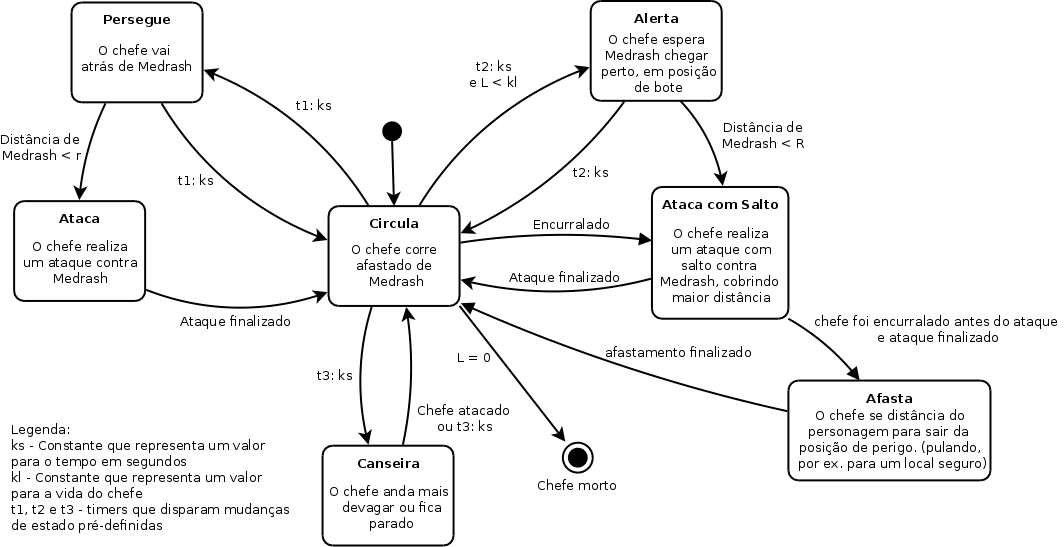
\includegraphics[scale=0.44]{ia_tigre.png}
 \caption{Máquina de estado do Tigre}
 \label{fsm:tigre}
\end{figure}

\subsection{Fase 2}

\subsubsection{Lobo}

O lobo fica patrulhando na montanha. Caso Medrash entre no raio de
deteção do lobo enquanto estiver com a tocha acesa, o lobo fugirá. Caso
Medrash entre no raio de deteção do lobo enquanto estiver com a tocha
apagada, o lobo perseguirá Medrash. Em qualquer um desses casos, se
Medrash ficar muito próximo do lobo, então o lobo atacará Medrash, e
voltará à atividade anterior.
Se, enquanto estiver sendo perseguido, Medrash acender a tocha,
o lobo fugirá. Similarmente, se o lobo estiver fugindo e a tocha se apagar,
o logo passará a perseguir Medrash.

\begin{figure}[!ht]
 \centering
 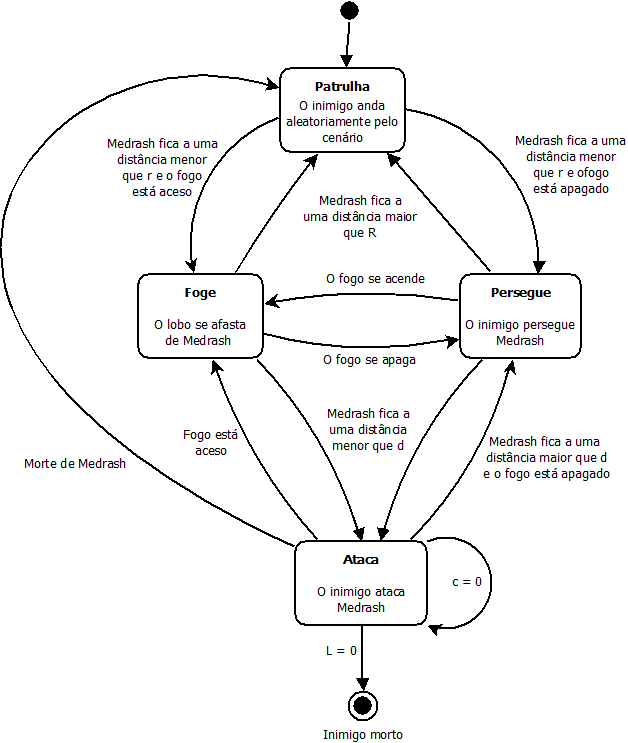
\includegraphics[scale=0.5]{ia_lobo.png}
 \caption{Máquina de estado do Lobo}
 \label{fsm:lobo}
\end{figure}

\subsubsection{Guerreiro}

O guerreiro entra no campo de batalha já perseguindo Medrash. Caso
Medrash esteja próximo do piromaníaco e dentro do raio de ataque do 
guerreiro, então o guerreiro empurrará Medrash.
Se Medrash não estiver muito próximo do piromaníaco, mas estiver dentro
do raio de ataque do guerreiro, então o guerreiro atacará Medrash.

\begin{figure}[!ht]
 \centering
 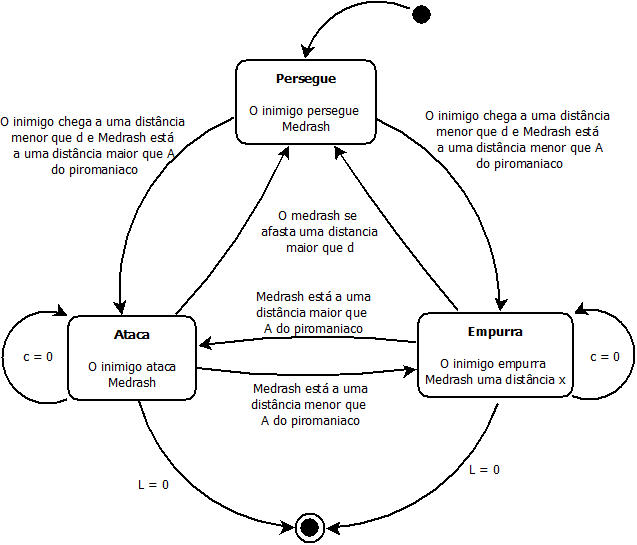
\includegraphics[scale=0.5]{ia_guerreiro.png}
 \caption{Máquina de Estado do Guerreiro}
 \label{fsm:guerreiro}
\end{figure}

\subsubsection{Piromaníaco}

O piromaníaco entra no campo de batalha se deslocando ao local mais
próximo para atear fogo. Seu único objetivo é atear fogo em todos os
locais possíveis. Caso isso aconteça, o jogador perde o jogo.

\begin{figure}[!ht]
 \centering
 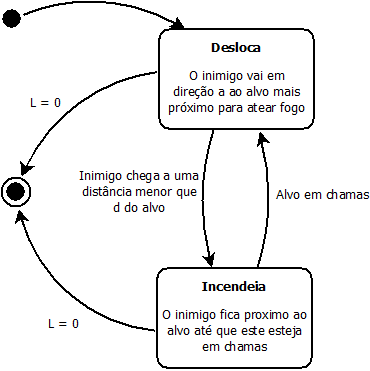
\includegraphics[scale=0.5]{ia_piromaniaco.png}
 \caption{Máquina de Estado do Piromaníaco}
 \label{fsm:piromaniaco}
\end{figure}

\subsection{Fase 3}

\subsubsection{Fanático}

O fanático será instanciado conforme necessário para atacar o Medrash.
Ele já inicia perseguindo Medrash. Quando fica perto o suficiente, ele
ataca Medrash. Se Medrash se afastar, ele volta a perseguí-lo.

\begin{figure}[!ht]
 \centering
 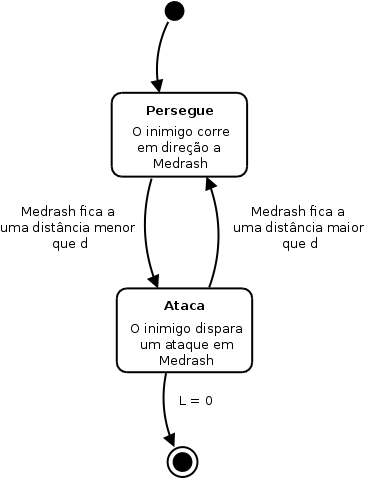
\includegraphics[scale=0.5]{ia_fanatico.png}
 \caption{Máquina de Estado do Fanático}
 \label{fsm:guerreiro}
\end{figure}

\subsubsection{Balasar (Chefe)}

O Balasar já inicia na batalha. Inicialmente ele prepara o ataque.
Após alguns segundos, ele investe em direção à Medrash. Seu movimento
é essencialmente retilíneo. Durante o movimento, sua rotação é limitada.
Se Balasar chegar a uma certa distância de Medrash durante a investida,
ele deferirá um ataque contra o mesmo. Medrash pode desviar desse ataque,
mas não pode se defender. Medrash pode fugir da investida, permanecendo
longe da trajetória de Balasar. Nesse caso, Balasar não realizará o ataque.
Depois da investida, bem sucedida ou não, Balasar se afastará.
Ao se afastar o suficiente, Balasar voltará a preparar o ataque.

Após uma certa quantidade de ataques, Balasar irá prender a clava no
chão. Nesse momento, Medrash deve ir atacar as estacas que prendem Sora.
Caso Medrash se aproxime de Balasar, ele será atacado com um chute que
também o afastará. Passado um certo período de tempo, Balasar solta a
clava, e volta a preparar o ataque.

\begin{figure}[!ht]
 \centering
 %\includegraphics[scale=0.5]{ia_balasar.png}
 \caption{Máquina de Estado do Balasar}
 \label{fsm:guerreiro}
\end{figure}

O objetivo de Medrash nessa batalha é libertar Sora, destruindo as 
estacas que a prendem. Quando Medrash destruir as estacas suficientemente,
Balasar mudará seu comportamento, se tornando mais agressivo.

Todos 